
\scsection{Методологические проблемы современного состояния работ в области Искусственного интеллекта}
\label{intro_ostis}

\begin{SCn}

\scnsectionheader{\currentname}

\scnstartsubstruct

\scnsegmentheader{Начало раздела "\currentname"}

\scnstartsubstruct

\scnheader{Методологические проблемы современного состояния работ в области Искусственного интеллекта}

\scnrelfromvector{конкатенация сегментов}
{Структура деятельности в области Искусственного интеллекта;}
\scnauthorcomment{дополнить список}

\scnrelfromset{рассматриваемые вопросы}{
\scnfileitem{Каковы основные стратегические цели (сверхзадачи) научно-технической деятельности в области \textit{Искусственного интеллекта}?};
\scnfileitem{Какие проблемы являются на сегодняшний день актуальными для дальнейшего развития различных направлений \textit{Искусственного интеллекта} и для развития \textit{Искусственного интеллекта} в целом как общей (объединённой) \textit{научно-технической дисциплины}, а также для развития различных форм деятельности в этой области (научно-исследовательской деятельности создания технологий разработки интеллектуальных компьютерных систем, образовательной деятельности, бизнеса)?};
\scnfileitem{Какие проблемы являются на сегодняшний день актуальными для развития других \textit{научно-технических дисциплин} и являются ли эти проблемы аналогичными тем, которые актуальны для развития \textit{Искусственного интеллекта}?};
\scnfileitem{Какие можно предложить подходы к решению указанных выше проблем и как для этого можно использовать создаваемый сейчас новый технологический уклад в области \textit{Искусственного интеллекта} (следующий уровень технологий искусственного интеллекта)?};
\scnfileitem{Как будет выглядеть на основе следующего уровня \textit{технологий Искусственного интеллекта} комплексная автоматизация вех \textit{видов человеческой деятельности}, а также взаимодействие различных \textit{видов человеческой деятельности}, т.е. как будет выглядеть архитектура \textit{smart-общества}?};
\scnfileitem{Устраивает ли нас уровень семантической совместимости взаимопонимания между современными виртуальными компьютерными системами и что необходимо сделать для повышения этого уровня?};
\scnfileitem{Устраивает ли нас уровень семантической совместимости взаимопонимания между современными интеллектуальными компьютерными системами их пользователями и что необходимо сделать для повышения этого уровня?}}
\scntext{аннотация}{Предлагаемое вашему вниманию рассмотрение методологических проблем современного состояния работ в области \textit{Искусственного интеллекта} состоит из следующих частей:
\begin{scnitemize}
\item Анализ актуальных проблем, препятствующих дальнейшему развитию  \textit{Искусственного интеллекта} как \textit{научно-технической дисциплины}:
\begin{scnitemizeii}
\item Проблемы развития научных исследований в области \textit{Искусственного интеллекта} 
\item Проблемы разработки технологий проектирования и реализации \textit{интеллектуальных компьютерных систем};
\item Проблемы формирования рынка \textit{интеллектуальных компьютерных систем}; 
\item Образовательные проблемы в области \textit{Искусственного интеллекта};
\item Проблемы развития бизнеса в области \textit{Искусственного интеллекта}.
\end{scnitemizeii}
\item Анализ проблем автоматизации сложных видов деятельности:
\begin{scnitemizeii}
\item научно-исследовательской деятельности в рамках различных научных дисциплин;
\item создание \textit{технологий проектирования} и производства (реализации) сложных технических систем;
\item \textit{инженерной деятельности} по разработке сложных технических систем;
\item \textit{образовательной деятельности} по наукоёмким техническим специальностям
\end{scnitemizeii}
\item Формулировка принципов, лежащих в основе \textit{Технологии OSTIS}, предназначенной для решения указанных выше проблем;
\item Рассмотрение структуры \textit{Экосистемы OSTIS}, построенной по \textit{Технологии OSTIS} и обеспечивающей комплексную автоматизацию всех видов человеческой деятельности
\end{scnitemize}}

\scnrelfromset{используемые знаки общих понятий и иных сущностей}{деятельность\\
\scnaddlevel{1}
\scnidtf{область деятельности}
\scnsuperset{человеческая деятельность}
\scnaddlevel{-1}
;вид деятельности\\
\scnaddlevel{1}
\scnhaselement{проектирование}
\scnaddlevel{1}
\scnidtf{проектная деятельность}
\scnaddlevel{-1}
\scnhaselement{производство}
\scnaddlevel{1}
\scnidtf{производственная деятельность}
\scnaddlevel{-1}
\scnhaselement{наука}
\scnaddlevel{1}
\scnidtf{научная деятельность}
\scnaddlevel{-2}
;проект\\
\scnaddlevel{1}
\scnsuperset{открытый проект}
\scnaddlevel{-1}
;консорциум
;технология\\
\scnaddlevel{1}
\scnsuperset{информационная технология}
\scnaddlevel{1}
\scnsuperset{технология искусственного интеллекта}
\scnaddlevel{-2}
;кибернетическая система\\
\scnaddlevel{1}
\scnsuperset{интеллектуальная система}
\scnaddlevel{1}
\scnsuperset{интеллектуальная компьютерная система}
\scnaddlevel{1}
\scnidtf{искусственная интеллектуальная система}
\scnaddlevel{-3}
;конвергенция\scnsupergroupsign
\scnaddlevel{1}
\scnidtf{уровень конвергенции (близости)}
\scnsuperset{конвергенция кибернетических систем\scnsupergroupsign}
\scnaddlevel{-1}
;интеграция*\\
\scnaddlevel{1}
\scnsuperset{интеграция кибернетических систем*}
\scnsuperset{эклектичная интеграция*}
\scnsuperset{глубокая интеграция*}
\scnaddlevel{-1}
;интегрированная система\\
\scnaddlevel{1}
\scnsuperset{эклектичная система}
\scnsuperset{гибридная система}
\scnaddlevel{-1}
;экосистема интеллектуальных компьютерных систем
;рынок знаний\\
\scnaddlevel{1}
\scnidtf{рыночная организация порождения эволюции и применения знаний}
\scnaddlevel{-1}
;smart-общество\\
\scnaddlevel{1}
\scnidtf{общество,в основе которого лежит экосистема интеллектуальных компьютерных систем и рынок знаний}
\scnaddlevel{-1}
}
 
\scnrelfromset{ключевые знаки}
{Искусственный интеллект\\
\scnaddlevel{1}
\scniselement{научно-техническая дисциплина}
\scnaddlevel{1}
\scnsubset{научно-техническая деятельность} 
\scnaddlevel{-2};
интеллектуальная система\\
\scnaddlevel{1}
\scnsuperset{интеллектуальная компьютерная система}
\scnaddlevel{-1};
Общая теория интеллектуальных систем;
Базовая комплексная технология проектирования интеллектуальных компьютерных систем;
Технология производства спроектированных интеллектуальных компьютерных систем;
Специализированная инженерия в области Искусственного интеллекта;
Образовательная деятельность в области Искусственного интеллекта;
Бизнес-деятельность в области Искусственного интеллекта\bigskip;
\scnkeyword{Технология OSTIS};
\scnkeyword{ostis-система};
смысловое преставление информации;
агентно-ориентированная модель обработки информации в памяти; стандартизация ostis-систем;
\scnkeyword{SC-код};
абстрактная sc-машина;
конвергенция знаний в памяти;
ostis-систем;
конвергенция моделей решения задач в  ostis-системе;
интеграция знаний в памяти  ostis-системы;
интеграция моделей решения задач в  ostis-системе;
ostis-сообщество;
ostis-технология\\
\scnaddlevel{1}
\scnsuperset{ostis-технология проектирования}
\scnsuperset{ostis-технология производства}
\scnsuperset{технология эксплуатации ostis-систем}
\scnsuperset{технология реинжиниринга ostis-систем}
\scnaddlevel{-1};
\scnkeyword{Ядро Технологии OSTIS}\bigskip;
OSTIS-портал научных знаний в области Искусственного интеллекта;
Проект IMS.ostis;
\scnkeyword{Метасистема IMS.ostis};
Проект Программной реализации универсальной абстрактной sc-машины;
Проект разработки Универсального sc-компьютера;
Специализированная инженерия, осуществляемая на основе Технологии OSTIS;
Образовательная деятельность в области Искусственного интеллекта, осуществляемая на основе технологии OSTIS;
\scnkeyword{Консорциум OSTIS}\bigskip;
\scnkeyword{Экосистема OSTIS};
человеческая деятельность;
вид человеческой деятельности;
автоматизация человеческой деятельности;
качество человеческой деятельности;
субъект Экосистемы OSTIS;
Рынок знаний, реализованный в рамках Экосистемы OSTIS;
smart-общество}

\scnendstruct

    При необходимости, \textit{ostis-система} может включать не только компоненты, разработанные на основе \textit{Технологии OSTIS}, но и легко интегрироваться с любыми другими системами и интегрировать другие компоненты посредством специального протокола обмена информацией и/или программного интерфейса (API). Такие компоненты не будут в полной мере обладать некоторыми важными свойствами ostis-систем (например, рефлексивностью) но это позволит заимствовать современные разработки и решить проблему производительности при решении наиболее ресурсоемких задач (например, при обучении нейросетей).
    }
\scnaddlevel{-1}
\scnnote{Важно отметить, что \uline{\textit{OSTIS} -- не конкретная интеллектуальная система} или способ решения задач какого-либо класса, это \uline{технология разработки интеллектуальных систем}, каждая из которых в свою очередь в каждый конкретный момент будет решать задачи определенного класса. При этом ключевые преимущества \textit{OSTIS} заключаются не в принципиально новых функциональных возможностях разрабатываемых систем (большинство \textit{ostis-систем} могут быть реализованы современными традиционными средствами), а в том, насколько легко можно \uline{модифицировать и развивать} разрабатываемые системы, адаптировать их под новые задачи, а также в том, насколько эффективно можно \uline{накапливать и использовать полученные компоненты} при разработке новых систем, снижая при этом сроки и трудоемкость их разработки.
}
\filemodetrue
\scnrelfromvector{текущий состав}{программная реализация платформы (модели семантического компьютера), которая лежит в основе каждой ostis-системы. Может использоваться как при разработке web-приложений, так и настольных и мобильных приложений.;
постоянно пополняемая \textit{Библиотека компонентов баз знаний ostis-систем}, включая универсальное \textit{Ядро баз знаний ostis-систем}. В текущий момент наличие данной библиотеки позволяет сократить сроки разработки баз знаний на 40-60\%.;
постоянно пополняемая \textit{Библиотека компонентов решателей задач ostis-систем}, включая механизмы поиска информации и некоторые модели решения задач, среди которых выделяется соответствующее \textit{Ядро решателей задач ostis-систем}. В настоящее время на первых этапах разработки системы оказывается достаточным использовать только \textit{Ядро решателей задач ostis-систем} и не разрабатывать дополнительно никаких компонентов.;
комплекс \textit{Средств информационной поддержки разработчиков ostis-систем} (включая описание самих моделей, а также методики и руководства), оформленных в виде интеллектуальной \textit{Метасистемы IMS.ostis} (IMS) и доступный онлайн \url{https://ims.ostis.net.}}

\scnrelfromvector{текущее применение}{на основе \textit{Технологии OSTIS} силами студентов и аспирантов активно развивается большое число открытых прототипов обучающих и справочных систем, которые можно найти на \url{https://github.com/ostis-apps};
разработки на основе \textit{Технологии OSTIS} успешно внедрены на ОАО ``Савушкин продукт''  при разработке системы информационного обслуживания сотрудников и при разработке компонентов систем контроля качества продукции;
\textit{Технология OSTIS} позволит значительно более эффективно реализовать анализ естественного языка (включая речь), в том числе для чат-ботов, синхронного перевода и речевых ассистентов. В настоящее время выполняется ряд проектов по данной тематике.}
\filemodefalse
\scntext{планы развития}{Предполагается, что в ближайшем будущем \textit{Метасистема IMS.ostis} и другие \textit{ostis-системы} будут объединены в распределенную облачную \textit{ostis-систему}, названную \textit{Экосистемой OSTIS}. Общая архитектура экосистемы показана на рисунке \textit{Архитектура Экосистемы OSTIS}. При этом все \textit{ostis-системы} в составе \textit{Экосистемы OSTIS} будут в каждый момент времени совместимы между собой, при этом совместимость будет контролироваться автоматически. Любой желающий сможет внести свой вклад в развитие любой из ostis-систем в составе \textit{Экосистемы OSTIS}, в первую очередь -- \textit{Метасистемы IMS.ostis}, при этом вклад будет автоматически верифицироваться и оцениваться. В то же время, как видно из представленной архитектуры, владельцы \textit{ostis-систем} смогут самостоятельно выбирать, какой частью своей информации они готовы поделиться с другими пользователями \textit{Экосистемы OSTIS}, персональная же часть информации будет гарантированно защищена.}

\scnheader{Архитектура Экосистемы OSTIS}
\scneqimage{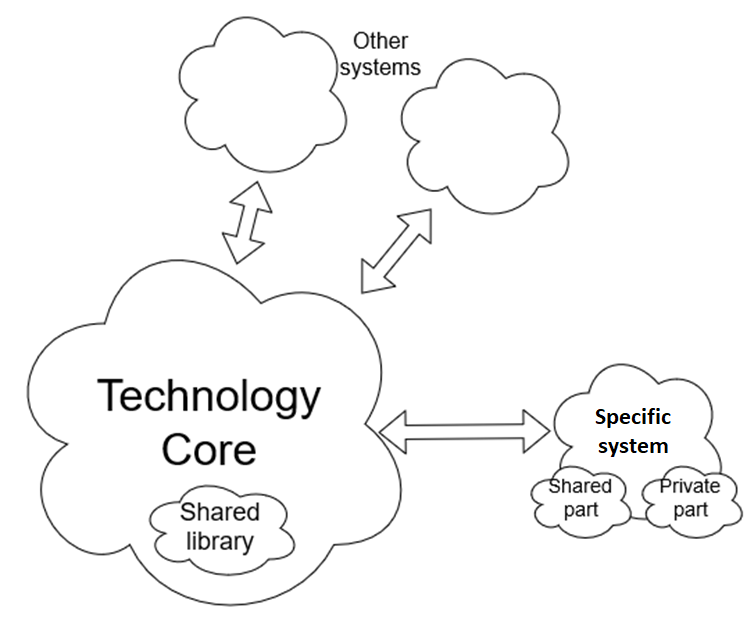
\includegraphics[width=0.6\textwidth]{figures/chapter0/ecosystem.png}}

\scnheader{Технология OSTIS}
\scnrelfromvector{текущие проекты}{Проект Экосистема OSTIS;Проект Метасистема IMS.ostis;Проект Семейство различных вариантов реализации универсального интерпретатора семантических моделей интеллектуальных систем\\
\scnaddlevel{1}
    \scnrelfromlist{подпроект}{Проект Программно реализованный на современных компьютерах универсальный интерпретатор семантических моделей интеллектуальных систем;Проект Семантический ассоциативный компьютер}
\scnaddlevel{-1}
;Проект Комплекс совместимых средств проектирования интеллектуальных систем\\
\scnaddlevel{1}
    \scnrelfromlist{подпроект}{Проект Встраиваемая типовая интеллектуальная система комплексной поддержки проектирования баз знаний;Проект Интеллектуальная система комплексной поддержки проектирования решателей задач интеллектуальных систем;Проект Интеллектуальная система комплексной поддержки проектирования вербальных интерфейсов интеллектуальных систем;Проект Интеллектуальная система комплексной поддержки проектирования невербальных интерфейсов}
\scnaddlevel{-1}
;Проект Семейство совместимых интеллектуальных справочных, обучающих и help-систем\\
\scnaddlevel{1}
    \scnrelfromlist{подпроект}{Проект Специализированные средства разработки совместимых интеллектуальных справочных, обучающих и help-систем различного назначения;Проект Комплекс семантически совместимых интеллектуальных справочных и обучающих систем по всем дисциплинам среднего образования;Проект Комплекс семантически совместимых интеллектуальных справочных и обучающих систем по всем дисциплинам, являющихся базовыми при подготовке инженеров по информационным специальностям;Проект Комплекс семантически совместимых интеллектуальных справочных и обучающих систем по всем специальным дисциплинам специальности ''Искусственный интеллект''{};Проект Семейство совместимых интеллектуальных справочных и обучающих систем по стандартам различного вида}
\scnaddlevel{-1}
;Проект Семейство совместимых интеллектуальных корпоративных систем ситуационного управления\\
\scnaddlevel{1}
    \scnrelfromlist{подпроект}{Проект Интеллектуальная корпоративная система ситуационного управления предприятием рецептурного производства;Проект Интеллектуальная корпоративная система ситуационного управления деятельностью выпускающей кафедры технического вуза}
\scnaddlevel{-1}
}
\scnrelfromvector{будущие проекты}{
Проект Семейство совместимых интеллектуальных систем автоматизации проектирования в различных областях;Проект Семейство совместимых порталов знаний\\
\scnaddlevel{1}
    \scnrelfrom{подпроект}{Проект Портал научных знаний по искусственному интеллекту}
\scnaddlevel{-1}
;Проект Семейство совместимых интеллектуальных систем экскурсионного обслуживания;Проект Семейство совместимых интеллектуальных геоинформационных систем;Проект Семейство совместимых интеллектуальных робототехнических систем и специализированных средств их разработки;Проект Семейство совместимых интеллектуальных систем персонального обслуживания и мониторинга\\
\scnaddlevel{1}
    \scnrelfromlist{подпроект}{Проект Интеллектуальная система персонального обслуживания и мониторинга пользователей и разработчиков компьютерных систем, входящих в Экосистему OSTIS;Проект Интеллектуальный персональный ассистент по взаимодействию с традиционными internet-системами и их пользователями;Проект Интеллектуальная система персонального комплексного медицинского мониторинга и контроля}
\scnaddlevel{-1}
}
\scnheader{конвергенция в области Искусственного интеллекта}

\scnrelfrom{разбиение}{Направления конвергенции в области Искусственного интеллекта}
     \scnaddlevel{1}
\scnhaselement{конвергенция Искусственного интеллекта со смежными научными дисциплинами}
    \scnaddlevel{1}
	\scnrelfrom{примечание}{\scnstartsetlocal\\
		\scnheaderlocal{Искусственный интеллект}
	\scnrelbothlist{смежная дисциплина}{Логика;Психология человека;Зоопсихология;Нейропсихология;Этология;Кибернетика;Общая теория систем;Семиотика;Лингвистика}
		\scnendstruct
	}
	\scnaddlevel{-1}

\scnhaselement{конвергенция различных направлений Искусственного интеллекта}
\scnaddlevel{1}
	\scnidtf{Конвергенция различных направлений исследований в области Искусственного интеллекта, результатом которой должна быть формализованная практически ориентированная общая теория интеллектуальных систем и, в частности, интеллектуальных компьютерных систем}
	\scnnote{Разобщенность различных направлений исследований в области искусственного интеллекта является главным препятствием создания общей комплексной технологии проектирования интеллектуальных компьютерных систем}
	\scnidtf{Конвергенция между различными направлениями и продуктами научных исследований в области искусственного интеллекта, результатом (целевым продуктом) которой должна стать общая формальная теория интеллектуальных компьютерных систем}
\scnaddlevel{-1}
\scnhaselement{конвергенция различного вида знаний в памяти интеллектуальной компьютерной системы}
\scnaddlevel{1}
	\scnidtf{Конвергенция и интеграция внутреннего представления в памяти интеллектуальной компьютерной системы различного вида знаний}
\scnaddlevel{-1}
\scnhaselement{конвергенция различных моделей решения задач в памяти интеллектуальной компьютерной системы}
\scnaddlevel{1}
	\scnidtf{Конвергенция и интеграция различных моделей решения задач, которая включает логико-семантическую типологию задач и типологию моделей решения задач и требует уточнения семантики таких понятий как задача, класс задач, метод, класс методов, модель решения задач (иерархический метод интерпретации класса методов)}
\scnaddlevel{-1}
\scnhaselement{конвергенция интеллектуальных компьютерных систем}
\scnaddlevel{1}
	\scnidtf{Обеспечение семантической совместимости (взаимопонимания) интеллектуальных систем, согласование используемых онтологий}
	\scnidtf{Конвергенция между различными прикладными компьютерными системами, результатом (целевым продуктом) которой должна стать экосистема, состоящая из перманентно эволюционирующих, семантически совместимых и взаимодействующих интеллектуальных компьютерных систем, а также их пользователей}
	\scnexplanation{Конвергенция (семантическая совместимость) всех разрабатываемых интеллектуальных компьютерных систем (в том числе прикладных), преобразующая набор индивидуальных (самостоятельных) интеллектуальных компьютерных систем различного назначения в коллектив активно взаимодействущих интеллектуальных компьютерных систем для совместного (коллективного) решения сложных (комплексных) задач и для перманентной поддержки семантической совместимости в ходе индивидуальной эволюции каждой интеллектуальной компьютерной системы.}
\scnaddlevel{-1}
\scnhaselement{конвергенция средств автоматизации проектирования различного вида компонентов интеллектуальных компьютерных систем}
\scnaddlevel{1}
	\scnidtf{Конвергенция (семантическая совместимость) средств автоматизации проектирования различного вида компонентов интеллектуальных компьютерных систем, результатом которой должен быть общий комплекс средств автоматизации проектирования всех компонентов интеллектуальных компьютерных систем}
	\scnidtf{Конвергенция между инструментальными средствами, обеспечивающими автоматизацию проектирования различных компонентов или различных классов интеллектуальных компьютерных систем, результатом (целевым продуктом) которой должен стать единый комплекс методологических и инструментальных средств, ориентированный на поддержку комплексного проектирования любых интеллектуальных компьютерных систем}
\scnaddlevel{-1}
\scnhaselement{конвергенция логико-семантических моделей интеллектуальных компьютерных систем}
\scnaddlevel{1}
	\scnnote{\textit{логико-семантические модели интеллектуальных компьютерных систем} являются результатом ("сухим"{} остатком) \textit{проектирования} этих систем и представляют собой формальное представления исходного (начального) состояния \textit{баз знаний} разрабатываемых \textit{интеллектуальных компьютерных систем}}
\scnaddlevel{-1}
\scnhaselement{конвергенция средств интерпретации логико-семантических моделей разрабатываемых интеллектуальных компьютерных систем}
\scnaddlevel{1}
\scnexplanation{Конвергенция (совместимость) средств реализации (производства) интеллектуальных компьютерных систем на основе спроектированных формальных моделей создаваемых интеллектуальных компьютерных систем (средств интерпретации спроектированных моделей интеллектуальных компьютерных систем). Такая интерпретация может осуществляться либо программным путем на современных компьютерах, либо путем создания принципиально новых компьютеров, специально ориентированных на интерпретацию формальных моделей интеллектуальных компьютерных систем, помещаемых в память указанных компьютеров}
\scnaddlevel{-1}
\scnhaselement{конвергенция между информационно-программным и 	аппаратным обеспечением интеллектуальных компьютерных систем}
\scnaddlevel{1}
	\scnidtf{Конвергенция между Software и Hardware интеллектуальных компьютерных систем}
\scnaddlevel{-1}
\scnhaselement{Конвергенция различных форм деятельности в области Искусственного интеллекта}
\scnaddlevel{1}
\scnexplanation{Конвергенция между
	\begin{scnitemize}
    \item научными исследованиями по созданию общей теории интеллектуальных компьютерных систем;
    \item разработкой средств автоматизации проектирования интеллектуальных компьютерных систем;
    \item разработкой средств интерпретации спроектированных формальных моделей интеллектуальных компьютерных систем;
    \item разработкой прикладных интеллектуальных компьютерных систем различного назначения;
    \item подготовкой и перманентным повышением квалификации кадров, способных эффективно участвовать во всех перечисленных направлениях деятельности.
    \end{scnitemize}
Глубокая конвергенция между всеми этими формами деятельности возможна только тогда, когда \uline{каждый} участник создания комплексной технологии искусственного интеллекта является участником \uline{каждой} из перечисленных форм деятельности.    
}
\scnidtf{Конвергенция между (1) научно-исследовательской деятельностью в области искусственного интеллекта; (2) инженерно-технологической деятельностью, которая направлена на разработку комплексной технологии проектирования интеллектуальных компьютерных систем и которая имеет высокий уровень наукоемкости; (3) инженерно-прикладной деятельностью, которая направлена на разработку прикладных интеллектуальных систем и которая также имеет высокий уровень наукоемкости, обусловленной необходимостью качественной формализации соответствующих предметных областей и, в частности, методов решения задач в этих областях; (4) образованием (образовательной деятельностью) в области искусственного интеллекта, повышение эффективности которого настоятельно требует раннего и поэтапного вовлечения студентов в реальные, а не учебные проекты - сначала в инженерно-прикладные, потом в инженерно- исследовательские проекты; (5) деятельностью, направленной на создание инфраструктуры, обеспечивающей поддержку открытого массового активного международного сотрудничества по консолидации усилий, направленных на решение современных проблем в области искусственного интеллекта; (6) бизнесом в области искусственного интеллекта, который не просто должен обеспечить финансовую поддержку перечисленных видов деятельности, но и обеспечить грамотный баланс между ними, грамотное сочетания тактических и стратегических целей}

\scnheader{Искусственный интеллект}
\scnrelfromset{методологические проблемы текущего состояния}{
\scnfileitem{Далеко не всеми учеными, работающими в области искусственного интеллекта принимается прагматичность практической направленности этой науки}
;\scnfileitem{Не всеми принимается необходимость конвергенции различных направлений искусственного интеллекта и необходимость их интеграции в целях построения общей теории интеллектуальных систем}
;\scnfileitem{Нет движения к построению общей компьютерной технологии интеллектуальных компьютерных систем}
;\scnfileitem{Нет движения к построению экосистем интеллектуальных компьютерных систем}
;\scnfileitem{Не всеми принимается необходимость конвергенции различных форм деятельности в области искусcтвенного интеллекта}}
\scnnote{Современная трактовка целей и задач Искусственного интеллекта как научно-технической дисциплины требует переосмысления, так как, к сожалению, носит несогласованный, а часто и значительно более узкий характер, чем этого требует текущее положение}


\scnheader{Бизнес-деятельность в области Искусственного интеллекта}
\scntext{текущее состояние}{Острая потребность в существенном повышении уровня автоматизации в самых различных областях человеческой деятельности (в промышленности, медицине, транспорте, образовании, строительстве и во многих других), а также современные результаты в развитии \textit{технологий Искусственного интеллекта} привели к существенному расширению работ по созданию \textit{прикладных интеллектуальных компьютерных систем} и к появлению большого количества коммерческих организаций, ориентированных на разработку таких приложений.}
\scnrelfromset{проблемы текущего состояния}{
\scnfileitem{Не так просто обеспечить баланс тактических и стратегических направлений развития всех форм деятельности в области \textit{Искусственного интеллекта} (научно-исследовательской деятельности, разработки технологии проектирования и производства интеллектуальных компьютерных систем, разработки прикладных систем, образовательной деятельности), а также баланс между всеми перечисленными формами деятельности.}
;\scnfileitem{В настоящее время отсутствует глубокая конвергенция различных форм деятельности в области \textit{Искусственного интеллекта} (в первую очередь, конвергенция развития технологий \textit{Искусственного интеллекта} и разработки различных прикладных интеллектуальных компьютерных систем), что существенно затрудняет развитие каждой из этих форм.}
;\scnfileitem{Высокий уровень наукоемкости работ в области \textit{Искусственного интеллекта} предъявляет особые требования к квалификации сотрудников и к их способности работать в составе творческих коллективов.}
;\scnfileitem{Для повышения квалификации своих сотрудников и для обеспечения высокого уровня своих разработок необходимо активное сотрудничество с различными научными школами, с кафедрами, осуществляющими подготовку молодых специалистов в области \textbf{\textit{Искусственного интеллекта}}, активное участие в подготовке и проведении соответствующих конференций, семинаров, выставок.}}

\scnheader{Искусственный интеллект}
\scnrelfromset{сверхзадачи текущего состояния}{
\scnfileitem{Построение и перманентное развитие \textit{общей формальной теории интеллектуальных систем}}
\scnaddlevel{1}
\scnrelfromset{подзадачи}{
\scnfileitem{Уточнение требований, предъявляемых к интеллектуальным компьютерным системам – уточнение свойств интеллектуальных компьютерных систем, определяющих высокий уровень их интеллекта.}
;\scnfileitem{Конвергенция и интеграция всевозможных видов знаний и всевозможных моделей решения задач в рамках каждой интеллектуальной компьютерной системы.}
;\scnfileitem{Ориентация на последующую разработку унифицированных семантически совместимых формальных моделей интеллектуальных систем.}
;\scnfileitem{Ориентация на разработку различного вида универсальных интерпретаторов формальных моделей интеллектуальных систем (и в том числе компьютеров нового поколения ) и обеспечение четкой стратификации между формальными моделями интеллектуальных систем и различными вариантами построения их интерпретаторов, обеспечивающей высокую степень независимости эволюции формальных моделей интеллектуальных систем и эволюции их интерпретаторов. Это требует особой детализации формальных моделей интеллектуальных систем.}
;\scnfileitem{Обеспечение коммуникационной ("социальной"{}) совместимости (договороспособности) интеллектуальных компьютерных систем, позволяющей им самостоятельно формировать коллективы интеллектуальных компьютерных систем и их пользователей, а также самостоятельно согласовывать (координировать) деятельность в рамках этих коллективов при решении сложных задач в непредсказуемых условиях. Без этого невозможна реализация таких проектов, как "умный"{} дом, "умный"{} город, "умное"{} предприятие, "умная"{} больница и т.д.}}
\scnaddlevel{-1}
;\scnfileitem{Создание и перманентное развитие \textit{общей комплексной технологии} проектирования и производства \textit{семантически совместимых} \scnbigspace \textit{интеллектуальных компьютерных систем}, способных координировать свою деятельность с себе подобными}
\scnaddlevel{1}
\scnrelfromset{подзадачи}{
\scnfileitem{Четкое описание стандарта интеллектуальных компьютерных систем, обеспечивающего семантическую совместимость разрабатываемых систем}
;\scnfileitem{Разработка мощных библиотек семантически совместимых и многократно (повторно) используемых компонентов разрабатываемых интеллектуальных компьютерных систем}
;\scnfileitem{Обеспечение низкого порога вхождения в технологию проектирования интеллектуальных компьютерных систем как для пользователей технологии (т.е. разработчиков прикладных или специализированных интеллектуальных компьютерных систем), так и для разработчиков самой технологии}
;\scnfileitem{Обеспечение высоких темпов развития технологии за счет учета опыта разработки различных приложений путем активного привлечения авторов приложений к участию в развитии (совершенствовании) технологии}}
\scnaddlevel{-1}
;\scnfileitem{Разработка компьютеров нового поколения, ориентированных на производство высокопроизводительных \textit{интеллектуальных компьютерных систем} самого различного назначения и высокого качества}
;\scnfileitem{Создание глобальной \textit{экосистемы} взаимодействующих между собой \textit{интеллектуальных компьютерных систем}, обеспечивающих комплексную автоматизацию всех \textit{видов человеческой деятельности}}
\scnaddlevel{1}
\scntext{подзадача}{Построение формальной модели человеческой деятельности в контексте теории smart-общества}
\scnaddlevel{-1}
;\scnfileitem{Создание и перманентное развитие глобальной \textit{социотехнической экосистемы}, которая состоит из \textit{интеллектуальных компьютерных систем}, а также всех пользователей этих систем, которая обеспечивает комплексную автоматизацию всех \textit{видов человеческой деятельности}}
;\scnfileitem{Необходим переход от эклектичного построения сложных \textit{интеллектуальных компьютерных систем}, использующих различные виды \textit{знаний} и различные виды \textit{моделей решения задач}, к их глубокой \textbf{интеграции} и унификации, когда одинаковые модели представления и модели обработки знаний реализуется в разных системах и подсистемах одинаково}
;\scnfileitem{Необходимо сократить дистанцию между современным уровнем \textbf{\textit{теории интеллектуальных компьютерных систем}} и практики их разработки.}}

\scnheader{Искусственный интеллект}
\scnidtf{Деятельность в области Искусственного интеллекта (как совокупность всех форм и направлений этой деятельности)}
\scntext{проблема текущего состояния}{Эпицентром современных проблем развития деятельности в области \textit{Искусственного интеллекта} является \textit{конвергенция} и \textit{глубокая интеграция} всех форм, направлений и результатов этой деятельности. Уровень взаимосвязи, взаимодействия и \textit{конвергенции} между различными формами и направлениями деятельности в области \textit{Искусственного интеллекта} явно недостаточен. Это приводит к тому, что каждая из них развивается обособленно, независимо от других.  Речь идет о \textit{конвергенции} между такими направлениями \textit{Искусственного интеллекта}, как представление знаний, решение интеллектуальных задач, интеллектуальное поведение, понимание и др., а также между такими формами \textit{человеческой деятельности в области Искусственного интеллекта}, как научные исследования, разработка технологий, разработка приложений, образование, бизнес. 
Почему на фоне уже достаточно длительного интенсивного развития научных исследований в области \textit{Искусственного интеллекта} до сих пор не создан рынок интеллектуальных компьютерных систем и комплексная технология \textit{Искусственного интеллекта}, обеспечивающая разработку широкого спектра \textit{интеллектуальных компьютерных систем} самого различного назначения и доступной широкому контингенту инженеров. 
Потому что сочетание высокого уровня наукоемкости и прагматизма этой проблемы требует для ее решения принципиально нового подхода к организации взаимодействия \textit{\uline{ученых}}, работающих в области \textit{Искусственного интеллекта}, \textit{\uline{разработчиков}} средств автоматизации проектирования \textit{интеллектуальных компьютерных систем}, \uline{\textit{разработчиков}} средств реализации интеллектуальных компьютерных систем, включая средства аппаратной поддержки интеллектуальных компьютерных систем, \uline{\textit{разработчиков}} прикладных интеллектуальных компьютерных систем. Такое \uline{целенаправленное} взаимодействие должно осуществляться как в рамках каждой из этих форм деятельности в области \textit{Искусственного интеллекта}, так и между ними. Таким образом, основной тенденцией дальнейшего развития теоретических и практических работ в области \textit{Искусственного интеллекта} является конвергенция как самых разных видов (форм и направлений) человеческой деятельности в области \textit{Искусственного интеллекта}, так и самых разных продуктов (результатов) этой деятельности. Необходимо ликвидировать барьеры между различными видами и продуктами деятельности в области \textit{Искусственного интеллекта} в целях обеспечения их совместимости и интегрируемости.
Проблема создания быстро развивающегося рынка семантически совместимых интеллектуальных систем – это вызов, адресованный специалистам в области \textit{Искусственного интеллекта}, требующий преодоления "вавилонского столпотворения"{} во всех его проявлениях, формирование высокой культуры договороспособности и унифицированной, согласованной формы представления коллективно накапливаемых, совершенствуемых и используемых знаний.
Ученые, работающие в области \textit{Искусственного интеллекта}, должны обеспечить конвергенцию результатов различных направлений \textit{Искусственного интеллекта} и построить: (1) общую теорию интеллектуальных компьютерных систем; (2) общую технологию проектирования семантически совместимых интеллектуальных компьютерных систем, включающую соответствующие стандарты интеллектуальных компьютерных систем и их компонентов. Инженеры, разрабатывающие интеллектуальные компьютерные системы, должны сотрудничать с учеными и участвовать в развитии технологии проектирования интеллектуальных компьютерных систем.}

\newpage
\scnsegmentheader{Текущее состояние и проблемы дальнейшего развития деятельности в области Искусственного интеллекта}
\scnstartsubstruct

\scntext{аннотация}{Рассмотрим в каких направлениях должна происходить эволюция повышенного качества деятельности в области \textit{Искусственного интеллекта}, а также эволюция продуктов этой деятельности}

\bigskip
\scnfragmentcaption

\scnheader{Научно-исследовательская деятельность в области Искусственного интеллекта}
\scntext{текущее состояние}{}
\scnauthorcomment{добавить из статей}

\scnheader{Научно-исследовательская деятельность в области Искусственного интеллекта}
\scnrelfromset{проблемы текущего состояния}{
\scnfileitem{Отсутствует согласованность систем \textit{понятий} в разных направлениях \textit{Искусственного интеллекта} и, как следствие, отсутствует \textit{семантическая совместимость} и \textit{конвергенция} этих направлений, в результате чего ни о каком движении в направлении построения \textit{общей теории интеллектуальных систем} с высоким уровнем формализации и речи быть не может. Существование и продолжающееся увеличение "высоты барьеров"{} между различными направлениями исследований в области \textit{Искусственного интеллекта} проявляется в том, что специалист, работающий в рамках какого-либо направления \textit{Искусственного интеллекта}, посещая заседания "не своей"{} секции на конференции по \textit{Искусственному интеллекту}, мало что там может понять и, соответственно, извлечь полезного для себя.};
\scnfileitem{Отсутствует мотивация и осознание острой необходимости в указанной \textit{конвергенции} между различными направлениями \textit{Искусственного интеллекта}.};
\scnfileitem{Отсутствует реальное движение в направлении построения \textit{Общей теории интеллектуальных систем}, поскольку отсутствует соответствующая мотивация и осознание острой практической необходимости в этом.}
}

\bigskip
\scnfragmentcaption

\scnheader{Разработка базовой комплексной технологии проектирования интеллектуальных компьютерных систем}
\scntext{текущее состояние}{Современная технология \textit{Искусственного интеллекта} представляет собой целое семейство всевозможных частных технологий, ориентированных на разработку и сопровождение различного вида компонентов \textit{интеллектуальных компьютерных систем}, реализующих самые различные модели представления и обработки информации, различные модели решения задач, ориентированных на разработку различных классов \textit{интеллектуальных компьютерных систем}.}
\scnrelfromset{проблемы текущего состояния}{
\scnfileitem{высокая трудоемкость разработки интеллектуальных компьютерных систем};
\scnfileitem{необходимая высокая квалификация разработчиков};
\scnfileitem{современные технологии \textit{Искусственного интеллекта} принципиально не обеспечивают разработки таких \textit{интеллектуальных компьютерных систем}, в которых устраняются недостатки современных \textit{интеллектуальных компьютерных систем}};
\scnfileitem{совместимость частных технологий \textit{Искусственного интеллекта} практически отсутствует и, как следствие, отсутствует \textit{семантическая совместимость} разрабатываемых \textit{интеллектуальных компьютерных систем}, поэтому их системная интеграция осуществляется \uline{вручную}.};
\scnfileitem{Разрабатываемые \textit{интеллектуальные компьютерные системы} не способны \uline{самостоятельно} координировать свою деятельность друг с другом следовательно
\begin{scnitemize}
\item{нет общей комплексной технологии проектирования интеллектуальных компьютерных систем};
\item{не обеспечивается совместимость и взаимодействие разрабатываемых систем (синтаксическая и семантическая совместимость)};
\item{нет совместимости между существующими частными технологиями проектирования различных компонентов интеллектуальных компьютерных систем (базы знаний, нейросетевые модели, интеллектуальные интерфейсы и т.д.)};
\item{есть инструментальные средства по компонентам, но "склеивать"{} (соединять, интегрировать) это надо вручную};
\item{нет системы инструментальных средств}
\end{scnitemize}
}
}

\bigskip
\scnfragmentcaption

\scnheader{Разработка технологии производства спроектированных интеллектуальных компьютерных систем}
\scntext{текущее состояние}{Был сделан целый ряд попыток разработки \textit{компьютеров} нового поколения, ориентированных на использование в \textit{интеллектуальных компьютерных системах}. Но все они оказались неудачными, так как не были ориентированы на всё многообразие моделей решения задач в \textit{интеллектуальных компьютерных системах}. В этом смысле они не были \textit{\uline{универсальными} компьютерами} для \textit{интеллектуальных компьютерных систем}.}
\scnrelfromset{проблемы текущего состояния}{
\scnfileitem{Разрабатываемые \textit{интеллектуальные компьютерные системы} могут использовать самые различные комбинации \textit{моделей решения интеллектуальных задач} (логических моделей, соответствующих различного вида логикам, нейросетевых моделей различного вида, моделей целеполагания, синтеза планов, моделей управления сложными объектами, моделей понимания и синтеза текстов естественного языка и т.д.). Современные (традиционные, фон-неймановские) \textit{компьютеры} не в состоянии достаточно производительно интерпретировать всё многообразие указанных моделей решения задач. При этом разработка специализированных \textit{компьютеров}, ориентированных на интерпретацию какой-либо одной модели решения задач (нейросетевой модели или какой-либо логической модели) проблему не решает, так как в \textit{интеллектуальной компьютерной системе} необходимо использовать сразу несколько разных моделей решения задач, причём в различных сочетаниях.}
}

\bigskip
\scnfragmentcaption

\scnheader{Специализированная инженерия в области Искусственного интеллекта}
\scnidtf{Деятельность, направленная на разработку \textit{интеллектуальных компьютерных систем} различного назначения с использованием имеющихся для этого моделей, методов и средств}
\scnidtf{Деятельность по проектированию и производству \textit{интеллектуальных компьютерных систем}}
\scnidtf{Деятельность, направленная на формирование рынка \textit{интеллектуальных компьютерных систем}}
\scnrelfrom{в перспективе}{Специализированная инженерия в области \textit{Искусственного интеллекта}, осуществляемая специальной частью Экосистемы OSTIS}
	\scnaddlevel{1}
	\scnrelfrom{продукт}{Экосистема OSTIS}
	\scnrelfrom{субъект действия}{часть Экосистемы OSTIS, осуществляющая специализированную инженерию в области \textit{Искусственного интеллекта}}
	\scnaddlevel{-1}

\scntext{текущее состояние}{}
\scnauthorcomment{добавить из статей}

\scnrelfromset{проблемы текущего состояния}{
\scnfileitem{Отсутствует четкая систематизация многообразия \textit{интеллектуальных компьютерных систем}, соответствующая систематизации автоматизируемых \textit{видов человеческой деятельности}.};
\scnfileitem{Отсутствует \textit{конвергенция} \scnbigspace \textit{интеллектуальных компьютерных систем}, обеспечивающих автоматизацию \textit{областей человеческой деятельности}, принадлежащих одному и тому же \textit{виду человеческой деятельности}.};
\scnfileitem{Отсутствует \textit{семантическая совместимость}(семантическая унификация, взаимопонимание) между \textit{интеллектуальными компьютерными системами}, основной причиной чего является отсутствие согласованной системы общих используемых \textit{понятий}.};
\scnfileitem{Семантическая недружественность \textit{пользовательского интерфейса} и отсутствие встроенной справочной системы, позволяющей запрашивать информацию об элементах интерфейса и возможностях системы, приводят к низкой эффективности эксплуатации всех возможностей \textit{интеллектуальной компьютерной системы}.};
\scnfileitem{Анализ проблем автоматизации всех \textit{видов человеческой деятельности} убеждает в том, что дальнейшая автоматизация \textit{человеческой деятельности} требует не только повышения уровня \textit{интеллекта} соответствующих \textit{интеллектуальных компьютерных систем}, но и реализации их способности
\begin{scnitemize}
\item устанавливать свою \textit{семантическую совместимость} (взаимопонимание) как с другими \textit{компьютерными системами}, так и со своими пользователями\char59
\item поддерживать эту \textit{семантическую совместимость} в процессе собственной эволюции, а также эволюции пользователей и других \textit{компьютерных систем}\char59
\item координировать свою деятельность с пользователями и другими \textit{компьютерными системами} при коллективно решении различных задач\char59
\item участвовать в распределении работ (подзадач) при коллективном решении различных задач.
\end{scnitemize}
Важно подчеркнуть то, что реализация вышеперечисленных способностей создаст возможность для существенной и даже полной автоматизации \textit{системной интеграции} \scnbigspace \textit{компьютерных систем} в комплексы взаимодействующих систем и автоматизации реинжиниринга таких комплексов. Такая автоматизация системной интеграции и её реинжиниринга:
\begin{scnitemize}
\item даст возможность комплексам кибернетических систем \uline{самостоятельно} адаптироваться к решению новых задач\char59
\item существенно повысит эффективность эксплуатации таких комплексов компьютерных систем, так как реинжиниринг системной интеграции компьютерных систем, входящих в такой комплекс, часто востребован (например, при реконструкции предприятия)\char59
\item существенно сокращает число ошибок по сравнению с "ручным"{} (неавтоматизированным) выполнением \textit{системной интеграции} и её \textit{реинжиниринга}, которые, к тому же, требует высокой квалификации.
\end{scnitemize}
Таким образом следующий этап повышения уровня автоматизации \textit{человеческой деятельности} настоятельно требует создания таких \textit{интеллектуальных компьютерных систем}, которые могли бы легко сами (без системного интегратора) объединяться для совместного решения сложных задач. 
}
}

\bigskip
\scnfragmentcaption

\scnheader{Образовательная деятельность в области искусственного интеллекта}
\scntext{текущее состояние}{Целенаправленная подготовка специалистов в области Искусственного интеллекта имеет богатую историю и осуществляется во многих ведущих университетах (Stanford University, MIT, МГУ (Москва), НИУ МЭИ (Москва), РГГУ (Москва), СПбГУ (Санкт-Петербург), ДВФУ (Владивосток), НГТУ (Новосибирск), НТУУ КПИ (Киев), БГУИР (Минск), БГУ (Минск), БрГТУ (Брест) и других).}
\scnrelfromset{проблемы текущего состояния}{
\scnfileitem{Поскольку деятельность в области \textit{Искусственного интеллекта} сочетает в себе и высокую степень наукоемкости и высокую степень сложности инженерных работ, подготовка специалистов в этой области требует одновременного формирования у них как научно-исследовательских навыков, культуры и стиля мышления, так и инженерно-практических навыков, культуры и стиля мышления. С точки зрения методики и психологии обучения сочетание фундаментальной научной и инженерно-практической подготовки специалистов является весьма сложный образовательной педагогической задачей.};
\scnfileitem{Отсутствует \textit{семантическая совместимость} между различными учебными дисциплинами, что приводит к "мозаичности"{} восприятия информации};
\scnfileitem{Отсутствует системный подход к подготовке молодых специалистов в области \textit{Искусственного интеллекта}};
\scnfileitem{Нет персонификации обучения};
\scnfileitem{Нет установки на выявление, раскрытие и развитие таланта творческого проектирования};
\scnfileitem{Отсутствует целенаправленное формирование мотивации к творчеству};
\scnfileitem{Нет формирования навыков работы в реальных коллективах разработчиков};
\scnfileitem{Отсутствует адаптация к реальной практической деятельности};
\scnfileitem{Любая современная технология (в том числе и Технология OSTIS) должна иметь высокие темпы своего развития, поскольку без этого невозможно поддерживать высокий уровень её конкурентоспособности. Но для быстро развиваемой технологии требуется:
\begin{scnitemize}
\item не просто высокая квалификация кадров, использующих и развивающих технологию,
\item но и высокие \uline{темпы} повышения уровня этой квалификации, так как без этого невозможно эффективно использовать и развивать \uline{быстро меняющуюся} технологию.
\end{scnitemize}
\bigskip
Из этого следует, что образовательная деятельность в области \textit{Искусственного интеллекта} и соответствующая ей технология должна быть не просто важной частью деятельности в области \textit{Искусственного интеллекта}, а частью, глубоко интегрированной во все остальные виды деятельности в области \textit{Искусственного интеллекта}. Так, например, каждая \textit{интеллектуальная компьютерная система} должная быть ориентирована не только на обслуживание своих конечных пользователей, не только на организацию целенаправленного взаимодействия со своими разработчиками, которые постоянно совершенствуют эту систему, и не только на обеспечение минимального "порога вхождения"{} для новых конечных пользователей и разработчиков, но и на организацию постоянного и персонифицированного повышения квалификации каждого своего конечного пользователя и разработчика в условиях постоянных изменений, вносимых в указанную \textit{интеллектуальную компьютерную систему}. Для этого эксплуатируемая \textit{интеллектуальная компьютерная система} должна "знать"{}, что в ней изменилось, на что она способна и как эти способности инициировать (содержание и форма, соответствующих пользовательских команд)
}
}

\scnendstruct
\scnendstruct

\scnheader{следует отличать*}
\scnhaselementset{
конвергенция
\scnaddlevel{1}
\scnidtf{Процесс сближения структурных и/или функциональных характеристик нескольких (как минимум двух) заданных сущностей}
\scnidtf{Процесс конвергенции заданных сущностей в ходе их изменения, совершенствование, эволюции}
\scnsubset{процесс}
\scnaddlevel{-1};
конвергенция\scnsupergroupsign 
\scnaddlevel{1}
\scnidtf{Степень близости (сходство) заданных сущностей}
\scniselement{свойство}
\scnaddlevel{-1}
}
\scnheader{конвергенция} 
\scnnote{ 
\textit{Конвергенция} пар конкретных искусственных сущностей (например, технических систем) есть стремление их унификацию (в частности, к стандартизации), т.е. стремление к минимизации многообразия форм решения аналогичных практических задач -- стремление к тому, чтобы все, что можно сделать одинаково, сделалось одинаково, но без ущерба требуемого качества. Последнее очень важно, так как безграмотная стандартизация может привести к существенному торможению прогресса. Ограничение многообразия форм не должно приводить к ограничению содержания, возможностей. Образно говоря, "словам должно быть тесно, а мыслям -- свободно".}
\scnnote{Методологически конвергенция искусственно создаваемых сущностей (артефактов) сводится (1) к выявлению (обнаружению) принципиальных сходств между этими сущностями, которые часто весьма закамуфлированы и их трудно "увидеть", и (2) к реализации обнаруженных сходств одинаковым образом (в одинаковой форме, в одинаковом "синтаксисе"). Образно говоря, от "семантической"{} (смысловой) эквивалентности требуется перейти и к "синтаксической" эквивалентности. Кстати, в этом как раз и заключается суть (идея) смыслового представления информации (знаний), целью которого является создание такой языковой среды (\textit{смыслового пространства}), в рамках которого (1) семантически эквивалентные информационные конструкции полностью совпадали, а (2) конвергенция информационных конструкций сводилась бы к выявлению изоморфных фрагментов этих конструкций.}
\scnnote{Очень важно уточнить, формализовать понятие конвергенции (конвергенции знаний, методов, модели решения задач, конвергенции интеллектуальных компьютерных систем в целом)}
\scnsuperset{конвергенция информационных конструкций}
\scnaddlevel{1}
\scnidtf{конвергенция синтаксических и семантических свойств информационных конструкций }
\scnaddlevel{-1}
\scnsuperset{конвергенция языков}
\scnsuperset{конвергенция научных дисциплин}
\scnaddlevel{1}
\scnidtf{конвергенция различных научных дисциплин или различных направлений одной и той же и дисциплины}
\scnaddlevel{-1}
\scnsuperset{конвергенция баз знаний}
\scnsuperset{конвергенция моделей решения задач}
\scnsuperset{конвергенция гибридных решателей задач}
\scnsuperset{конвергенция кибернетических систем}
\scnsuperset{конвергенция интеллектуальных систем}
\scnaddlevel{1}
\scnsuperset{конвергенция интеллектуальных систем, направленная на обеспечение их \uline{семантической совместимости}}
\scnaddlevel{-1}

\scnheader{конвергенция результатов научно-технической деятельности}
\scnnote{Важным препятствием для конвергенции результатов научно-технической деятельности является сформировавшийся в науке и технике акцент на выявлении не сходств, а отличий. Чтобы убедиться в этом достаточно обратить внимание на то, что уровень научных результатов оценивается научной \uline{новизной}, которая может имитироваться новизной не по существу, а по форме представления (например, с помощью новых понятий или даже новых терминов). Результаты в технике, например, в патентах также оцениваются \uline{отличиями} от предшествующих технических решений. Но для конвергенции нужны другие акценты -- ни поиск отличий, а выявление неочевидных сходств и превращения их в очевидные сходства, представленные в одинаковой \uline{форме}.}

\scnheader{совместимость\scnsupergroupsign}
\scnidtf{совместимость заданных двух или более сущностей\scnsupergroupsign}
\scnidtf{простота интеграции заданной группы сущностей\scnsupergroupsign}
\scnidtf{интегрируемость\scnsupergroupsign}
\scnnote{Степень (уровень) совместимости заданных сущностей может рассматриваться как оценка результата их конвергенции. Чем качественнее (основательнее, глубже) проведена конвергенция заданных сущностей, тем выше уровень их совместимости и, собственно, тем легче их интегрировать.}

\scnsuperset{cовместимость информационных конструкций\scnsupergroupsign}
\scnaddlevel{1}
\scnsuperset{семантическая совместимость информационных конструкций\scnsupergroupsign}
\scnaddlevel{-1}
\scnsuperset{совместимость языков\scnsupergroupsign}
\scnaddlevel{1}
\scnsuperset{семантическая совместимость языков\scnsupergroupsign}
\scnaddlevel{-1}
\scnsuperset{семантическая совместимость научных дисциплин\scnsupergroupsign}
\scnsuperset{совместимость баз знаний\scnsupergroupsign}
\scnsuperset{совместимость моделей решения задач\scnsupergroupsign}
\scnsuperset{совместимость кибернетических систем\scnsupergroupsign}
\scnaddlevel{1}
\scnsuperset{семантическая совместимость кибернетических систем\scnsupergroupsign}
\scnaddlevel{-1}
\scnsuperset{семантическая совместимость\scnsupergroupsign}

\scnheader{интеграция*}
\scnidtf{объединение нескольких разных сущностей, в результате чего возникает некоторая объединённая целостная сущность*}
\scnsuperset{эклектичная интеграция*}
\scnaddlevel{1}
\scnidtf{Интеграция разнородных (гетерогенных) сущностей, которой не предшествует конвергенция (сближение) этих сущностей*}
\scnaddlevel{-1}
\scnsuperset{глубокая интеграция*}
\scnnote{Понятие \textit{интеграции*} и особенно понятие \textit{глубокой интеграции*} имеет тесную связь с понятием \textit{конвергенции\scnsupergroupsign}. Чем выше степень конвергенции (степень сближения) интегрируемых объектов, тем выше качество результата интеграции. Особенно, если речь идёт о глубокой интеграции.}

\scnheader{глубокая интеграция*}
\scnidtf{"бесшовная"{} интеграция*}
%TODO ссылка на Грибову
\scnidtf{интеграция однородных сущностей, предполагающая глубокую взаимную "диффузию"{} (сращивание) соединяемых сущностей, которая не обязательно должна осуществляться физически}
\scnnote{Примером виртуальной глубокой интеграции является формирование коллектива \uline{семантический совместимых} индивидуальный кибернетических систем}
\scnidtf{бесшовная интеграция*}
\scnidtf{гибридизация*}
\scnidtf{интеграция, результатом которой являются гибридные объекты*}
\scnidtf{интеграция, которой предшествует высокий уровень конвергенции интегрируемых объектов*}
\scnidtf{(конвергенция + интеграция)*}
\scnidtf{"бесшовная"{} интеграция}
\scnidtf{интеграция, в результате которой возникает гибридная система*}
\scnidtf{интеграция, которой предшествует конвергенция (в частности, унификация) интегрируемых систем, приведение этих систем к максимально похожему виду (общему знаменателю)*}
%TODO сложно при чтении воспринимать, конвергенция и приведение как-то сливаются, становится не совсем понятно, к чему относится приведение к конвергенции или к интеграции, может как-то более явно указать, что конвергенция это то приведение?
\scnidtf{интеграция с "диффузией"{} , взаимопроникновением на основе унификации того, что можно сделать одинаковым*}

\scnheader{интеграция*}
\scnsuperset{интеграция информационных конструкций}
\scnsuperset{интеграция языков}
\scnsuperset{интеграция научных дисциплин}
\scnsuperset{интеграция баз знаний}
\scnsuperset{интеграция моделей решения задач}
\scnsuperset{интеграции индивидуальных кибернетических систем}
\scnaddlevel{1}
\scnsuperset{слияние индивидуальных кибернетических систем}
\scnaddlevel{1}
\scnidtf{преобразование нескольких \uline{искусственных} индивидуальных кибернетических систем в интегрированную индивидуальную кибернетическую систему, которая способна решать все задачи, каждая из которых могла бы быть решена в рамках какой-либо из интегрируемых систем}
\scnaddlevel{-1}
\scnsuperset{формирование коллектива индивидуальных кибернетических систем}
\scnaddlevel{1}
\scnidtf{формирования многоагентной системы, состоящей из индивидуальных кибернетических систем}
\scnaddlevel{-1}
\scnnote{Эффективность интеграции индивидуальных кибернетических систем определяется тем, насколько объем задач, решаемых коллективом индивидуальных кибернетических систем, превысит объединение объёмов задач, решаемых членами коллектива в отдельности.}
\scnaddlevel{-1}

\bigskip
\scnendstruct \scninlinesourcecommentpar{Завершили Сегмент "\textit{Текущее состояние и проблемы дальнейшего развития деятельности в области Искусственного интеллекта}"}

\end{SCn}
